\section{Data}\label{data}

The dataset used in this shared task is the \ArgKP dataset~\cite{Bar-HaimEFKLS2020} which consists of 24\,083 argument 
and key point pairs labeled as matching/non-matching. They all belong to one of 28~controversial topics, for example: 
\textquote{Assisted suicide should be a criminal offence}. Every pair has a stance towards the topic. 

The split used for training has 5\,583~arguments belonging to 207~key points within 24~topics. This leaves the 
validation dataset with 932~arguments and 36~key points for 4~topics. The test split, used for evaluation of 
all submissions, contains 723~arguments with 33~key points. There are 3~topics given in the test dataset.

\subsection{Characteristics}
\begin{table*}
    \caption{Examples of \todo{matching} argument key point pairs from the \ArgKP dataset~\cite{Bar-HaimEFKLS2020}}
    \label{examples}
    \begin{tabularx}{\linewidth}{lXp{4.3cm}c}
      \toprule
      \textbf{\#} & \textbf{Argument} & \textbf{Key point} \\
      \midrule
      A & % from training set, match
      child \textcolor{violet}{actors} can be overworked and they can miss out on their education. & % arg_13_153
      Being a \textcolor{violet}{performer} harms the child's education \\ % kp_13_5
      B & % from training set, match
      as long as nuclear weapons exist, the entire world has to worry about \textcolor{violet}{nations} deciding to fire them at another or \textcolor{violet}{terrorists} getting hold of them and causing disaster & % arg_17_91	
      Nuclear weapons can fall into the \textcolor{violet}{wrong hands} \\ % kp_17_1
      C & % from training set, not labelled
      `people reach their limit when it comes to their quality of life and should be able to end their \textcolor{violet}{suffering}. this can be done with little or no \textcolor{violet}{suffering} by \textcolor{teal}{assistance} and the person is able to say good bye. & % arg_0_0
      \textcolor{teal}{Assisted} suicide reduces \textcolor{violet}{suffering} \\ % kp_0_1
      \bottomrule
    \end{tabularx}
  \end{table*}


Analyzing the data, shows that matched and unmatched key points of a given argument contain a certain proportion of the same words. 
Many of these are stopwords such as \textquote{as}, \textquote{for}, and \textquote{not} and are a well known problem 
in Natural Language Processing.
Stopwords are redundant and uniformative and thus should not influence token overlap.
We therefore remove stop words from our data during preprocessing to avoid such a problem. 
Furthermore, important words found in arguments are repeated with different tenses and parts of speech in key points, for example: 
\textquote{legalize}, \textquote{legalized}, \textquote{legalizing}, \textquote{legal}. 
To achieve an unambiguous spelling, such words are normalized with a stemming method in our approach. 
%This conversion to the word root reduces the size of the vocabulary or the dimensions of the text input.

In Table~\ref{examples} we show examples of argument key point pairs from the \ArgKP dataset~\cite{Bar-HaimEFKLS2020}. 
We identify the following major difficulties in matching key points to arguments: semantically similar words and meaning 
understanding.
In example pair~A from Table~\ref{examples}, the key point can be matched with its argument. Both sentences discuss 
children actors and their education. The word \textquote{actors} is not explicitly used in the key point but is 
semantically similar to the word \textquote{performer}. 
In our approach we oppose this challenge by using the well-known lexical database WordNet~\cite{Miller1995} in our 
baseline to find synonyms and antonyms.
In example~B from Table~\ref{examples}, argument and key point are expressed differently. 
The key point makes usage of \textquote{wrong hands} as figurative meaning for \textquote{nations} and \textquote{terrorists} from the argument. 
To predict if a key point is aligned with some argument, we need to understand their meanings and compare them. 
To better deal with this problem, we use two well-known language models in our second approach~(Section~\ref{approach}). 

\begin{figure*}
    \centering
    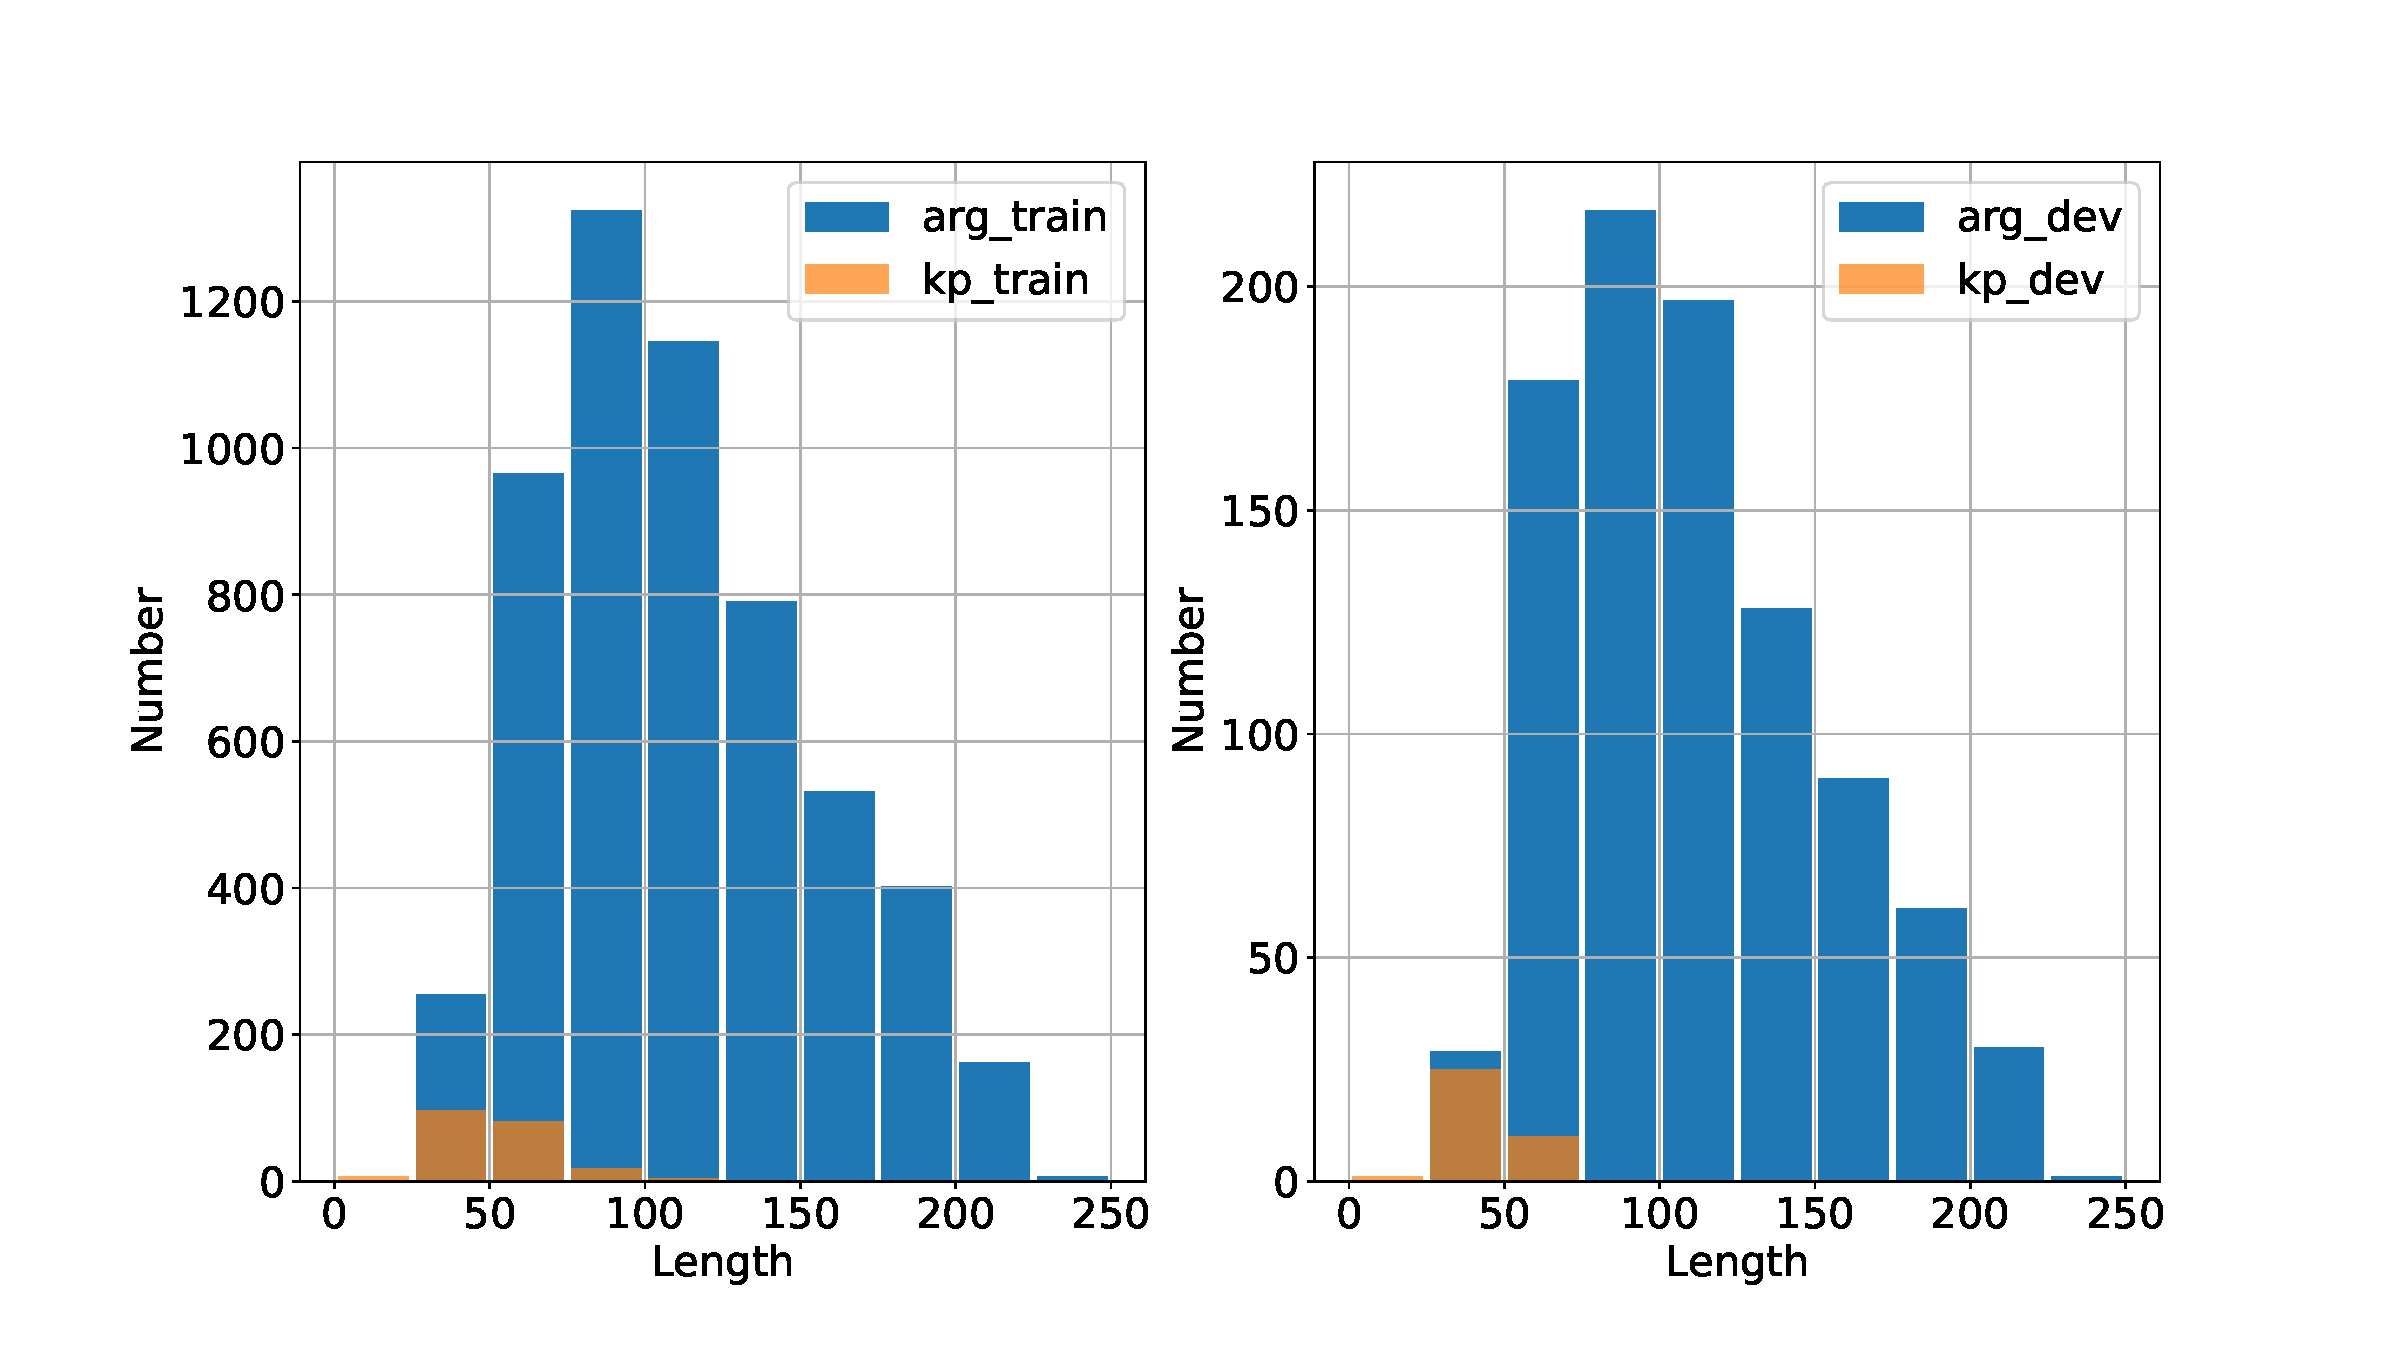
\includegraphics[width=\linewidth]{arg-kp-length.pdf}
    \label{arg-kp-length}
    \caption{Differences in argument and key point lengths in the training and development set.}
\end{figure*}

We make another observation, that arguments in both datasets are longer than the key points. As can be seen in Figure~\ref{arg-kp-length}. 
The average length of arguments is about 109~tokens. Compared to that, key points are, on average, only half as long with 51.7~tokens.
An argument can be supported by several key points. This set of all matching key points can be called the summary of the given argument.  
In the validation dataset, the key points have an average length of 41.3~tokens and therefore less than in the training dataset. 
The average length of arguments remains almost the same at 107~tokens. 
We have an average length of 7.5~characters for tokens in the training split and 7~characters in the validation split. 
The differences in length between arguments and key points from the training dataset and validation dataset are 57.8 and 66.3 respectively. 
This means that the arguments from the training dataset are, on average, 7.6~tokens longer than the key points and 
in the validation dataset this increases to about 9.5~tokens. 
From this, we concloude that long arguments in the validation set are summarised stronger than arguments from the training set. 
The proportion of arguments that are more than 66.3~letters longer than key points is about 39~\% of the training set 
and about 44~\% of the validation set. 
We can see that there are more long arguments in the validation set. 
We analyze the effect of this characteristic on the classification model further by results and error analysis~(Section~\ref{error-analysis}).
